\chapter{Simulations}

\section{Solenoid tilt angle and its effect on the $B_z$ field peaks}
\label{sec:simulations}

To further understand why the model presented in equation
\ref{eq:angle_estimation} did not perform as hoped, the relationship
between the $B_z$ field peaks and the yaw angle was investigated in
a simulation campaign. The coil dimensions presented in figure
\ref{fig:sim-mag-dims} were varied in a parametric sweep.
For each sweep, the $z$ value at the field maximum along the lines $l_1$ and $l_2$
was calculated as a function of the yaw angle \emph{Rot}. Each
of the lines were tangential to the $z$ axis with some offset
$y_{off}$ in $y$ as presented in figure \ref{fig:sim-mag-rot}.

\begin{figure}[h!]
    \centering
    \begin{subfigure}[b]{0.4\textwidth}
        \centering
        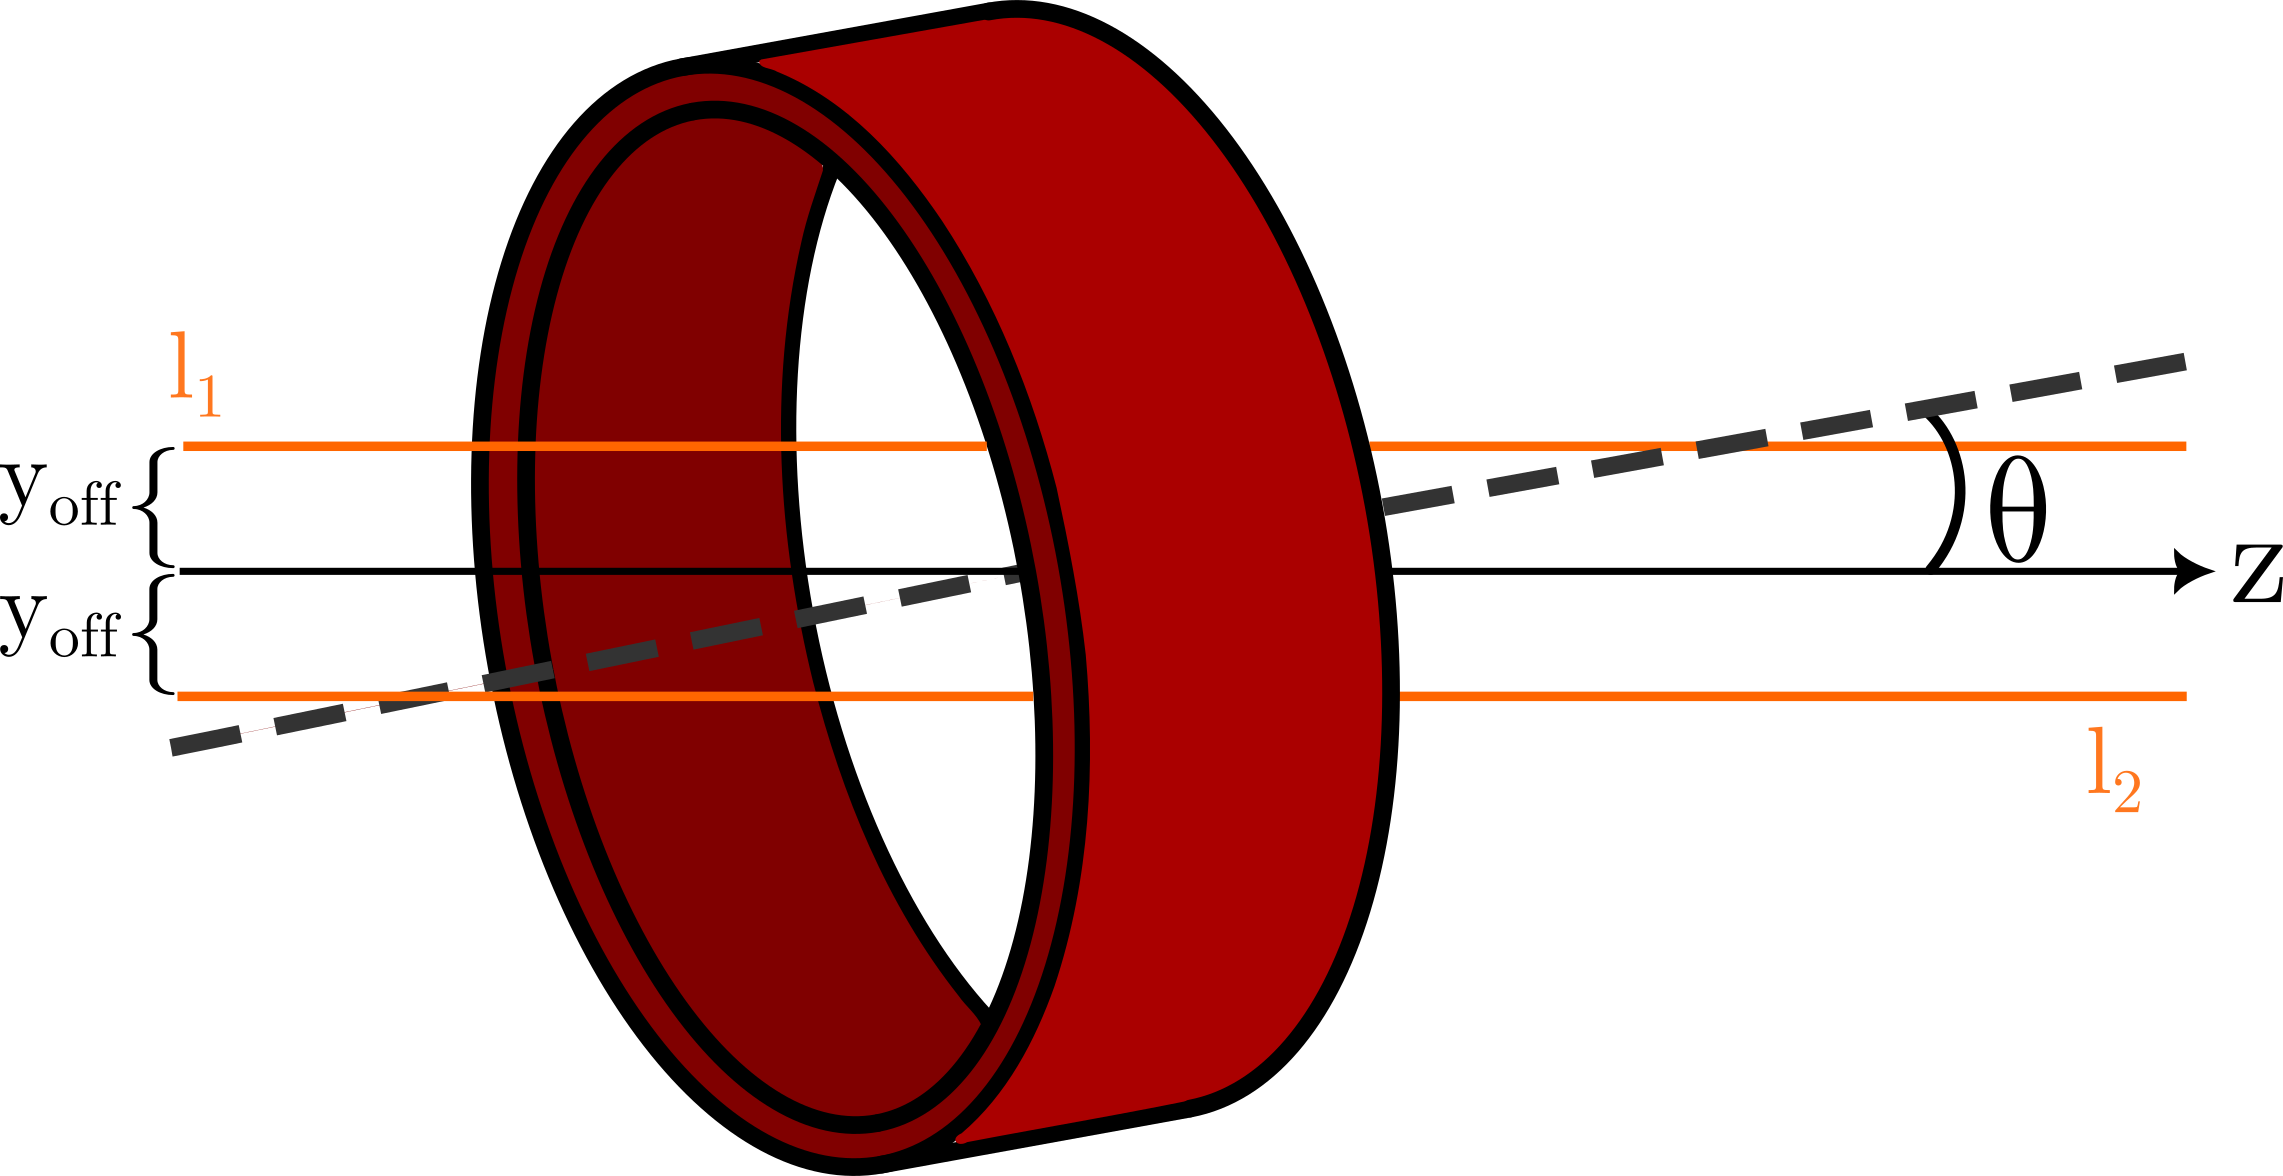
\includegraphics[height=100pt]{figs/sim_mag_rot}
        \caption{Coil placement parameters in simulations.}
        \label{fig:sim-mag-rot}
    \end{subfigure}
    \hfill
    \begin{subfigure}[b]{0.4\textwidth}
        \centering
        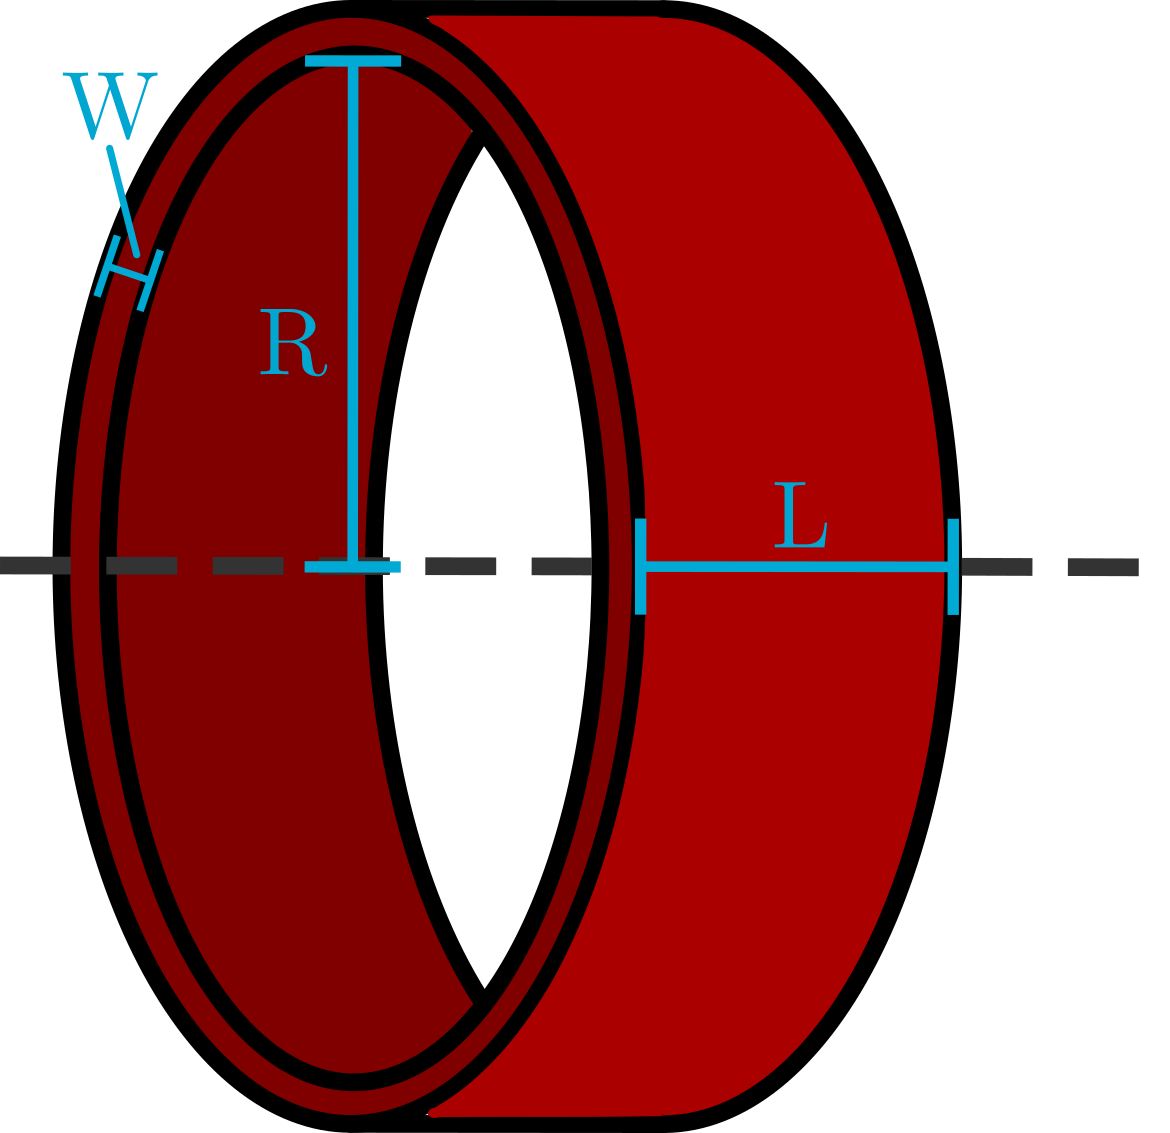
\includegraphics[height=100pt]{figs/sim_mag_dims}
        \caption{Coil dimension parameters in simulations.}
        \label{fig:sim-mag-dims}
    \end{subfigure}
    \caption{}
\end{figure}

The range and unique values for each parameter is presented in table \ref{tab:parameter-vals}.
The parameter values are spaced out evenly across their range. Where necessary, simulation
results have been discarded when the $y$ offsets are too large, such that the lines $l_1$
and $l_2$ go through the numerical singularities inside the magnet.

\begin{table}[h!]
    \begin{center}
        \begin{tabular}{c c c c}
            Parameter              & Shorthand name & Range         & \#Unique Values \\
            \hline
            Magnet Radius          & \emph{R}       & $0.2-0.5$ m   & 21              \\
            Magnet Width/Thickness & \emph{W}       & $0.0-0.4$ m   & 6               \\
            Magnet Length          & \emph{L}       & $0.0-0.5$ m   & 9               \\
            Line $y$ offset        & $y_{off}$      & $0.05-0.2$ m  & 11              \\
            Magnet yaw angle       & \emph{Rot}     & $0.0-0.5$ rad & 31
        \end{tabular}
        \caption{Simulation parameter values}
        \label{tab:parameter-vals}
    \end{center}
\end{table}

The simulations were done numerically, with several thin
current loops spread out at a constant density along the magnet
width $W$ and length $L$. Some randomly chosen results were
verified using FEM simulations with a similar magnet model.

Figure \ref{fig:sim-mag-dimensions} gives an idea of the general impact that the
magnet dimensions have on the peak shifts. For each plot, the other magnet dimensions
are constant. A key takeaway is that most magnet dimensions do not affect
the peak shift that much at the chosen parameter values, especially at 
lower yaw angles. The offset from the axis however has a great effect.


\begin{figure}
    \centering
    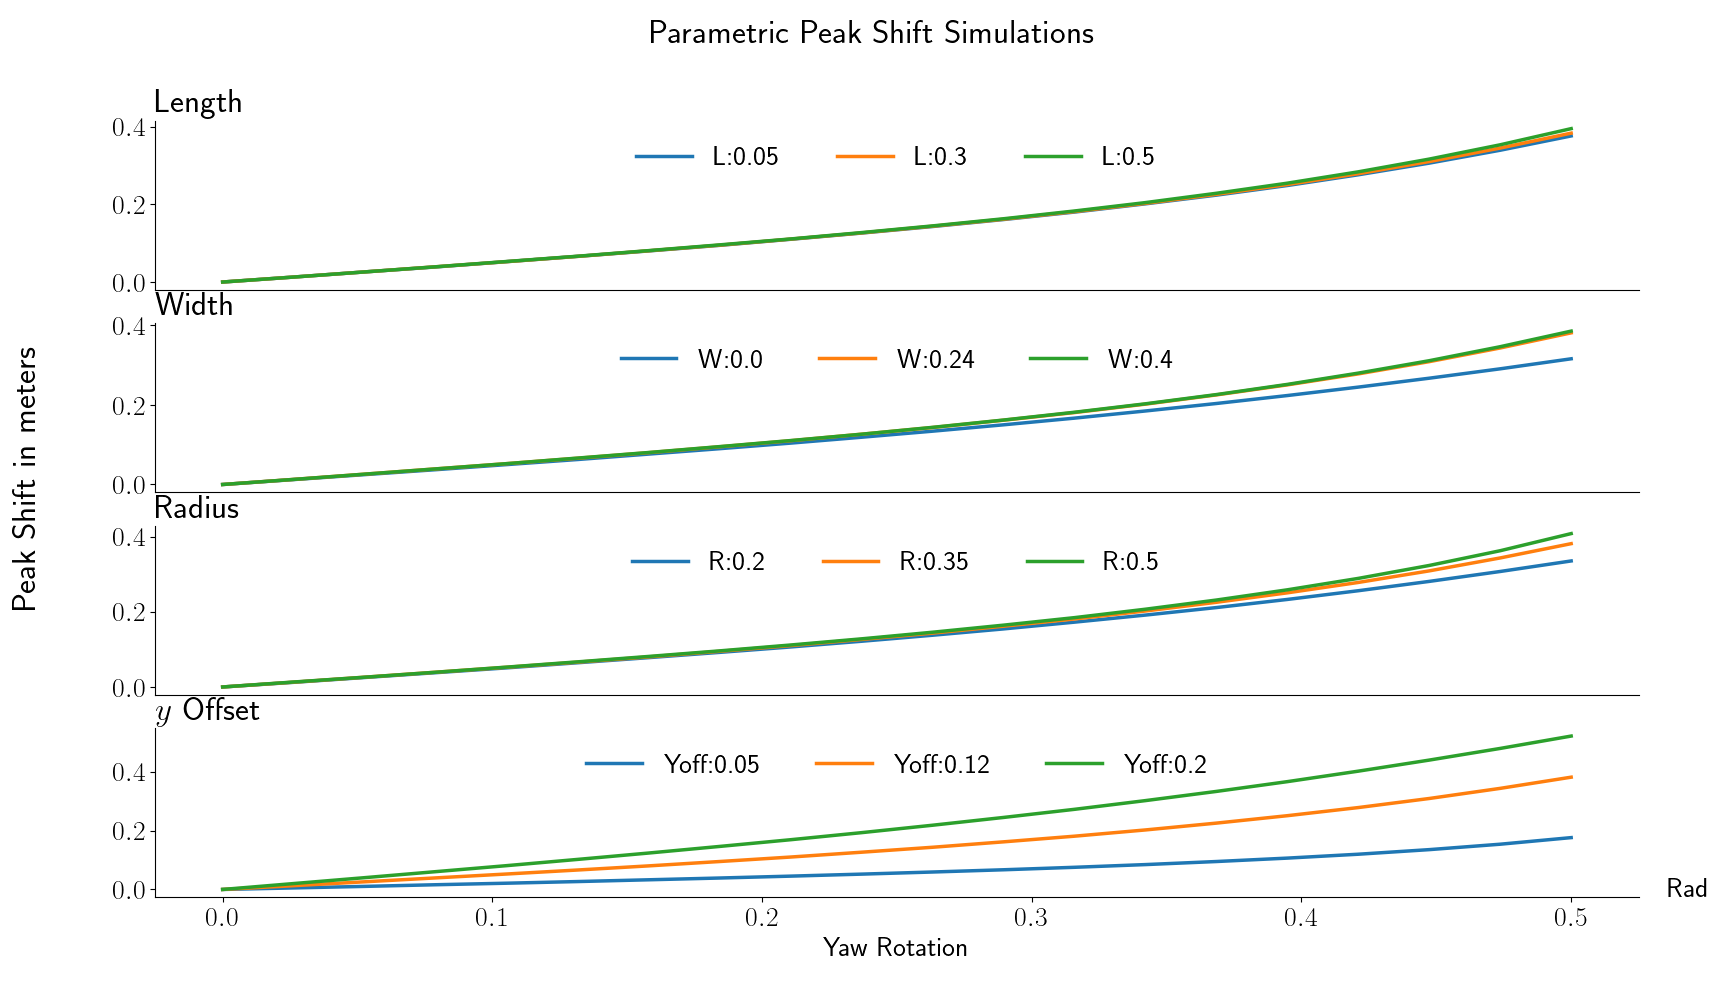
\includegraphics[width=\linewidth]{figs/sim_params_plot}
    \caption{Peak shifts and how they vary with yaw angle and magnet dimensions.}
    \label{fig:sim-mag-dimensions}
\end{figure}

The effect of the $y$ offset can be clearly seen in figure
\ref{fig:sim-mag-fieldmap-argmax}. Unfortunately, it does not seem
that the effect is easily modeled. For a simple current loop, the peak 
shifts could be modeled by fitting the maxes to some tangent function
in $y$, but for more realistic magnet models, discontinuites are present as
the $y$ offset approaches the magnet ends. These discontinuites are
likely not measurable in practice though, being too close or even
inside the windings.
Clearly, the simple model
presented in equation \ref{eq:angle_estimation} will overestimate
the angle since the $B_z$ peaks are not distributed along the geometric
solenoid centre, but rather further out. The $\Delta z$ argument in
equation \ref{eq:angle_estimation} will thus be larger than the model 
expects.


\begin{figure}[h!]
    \centering
    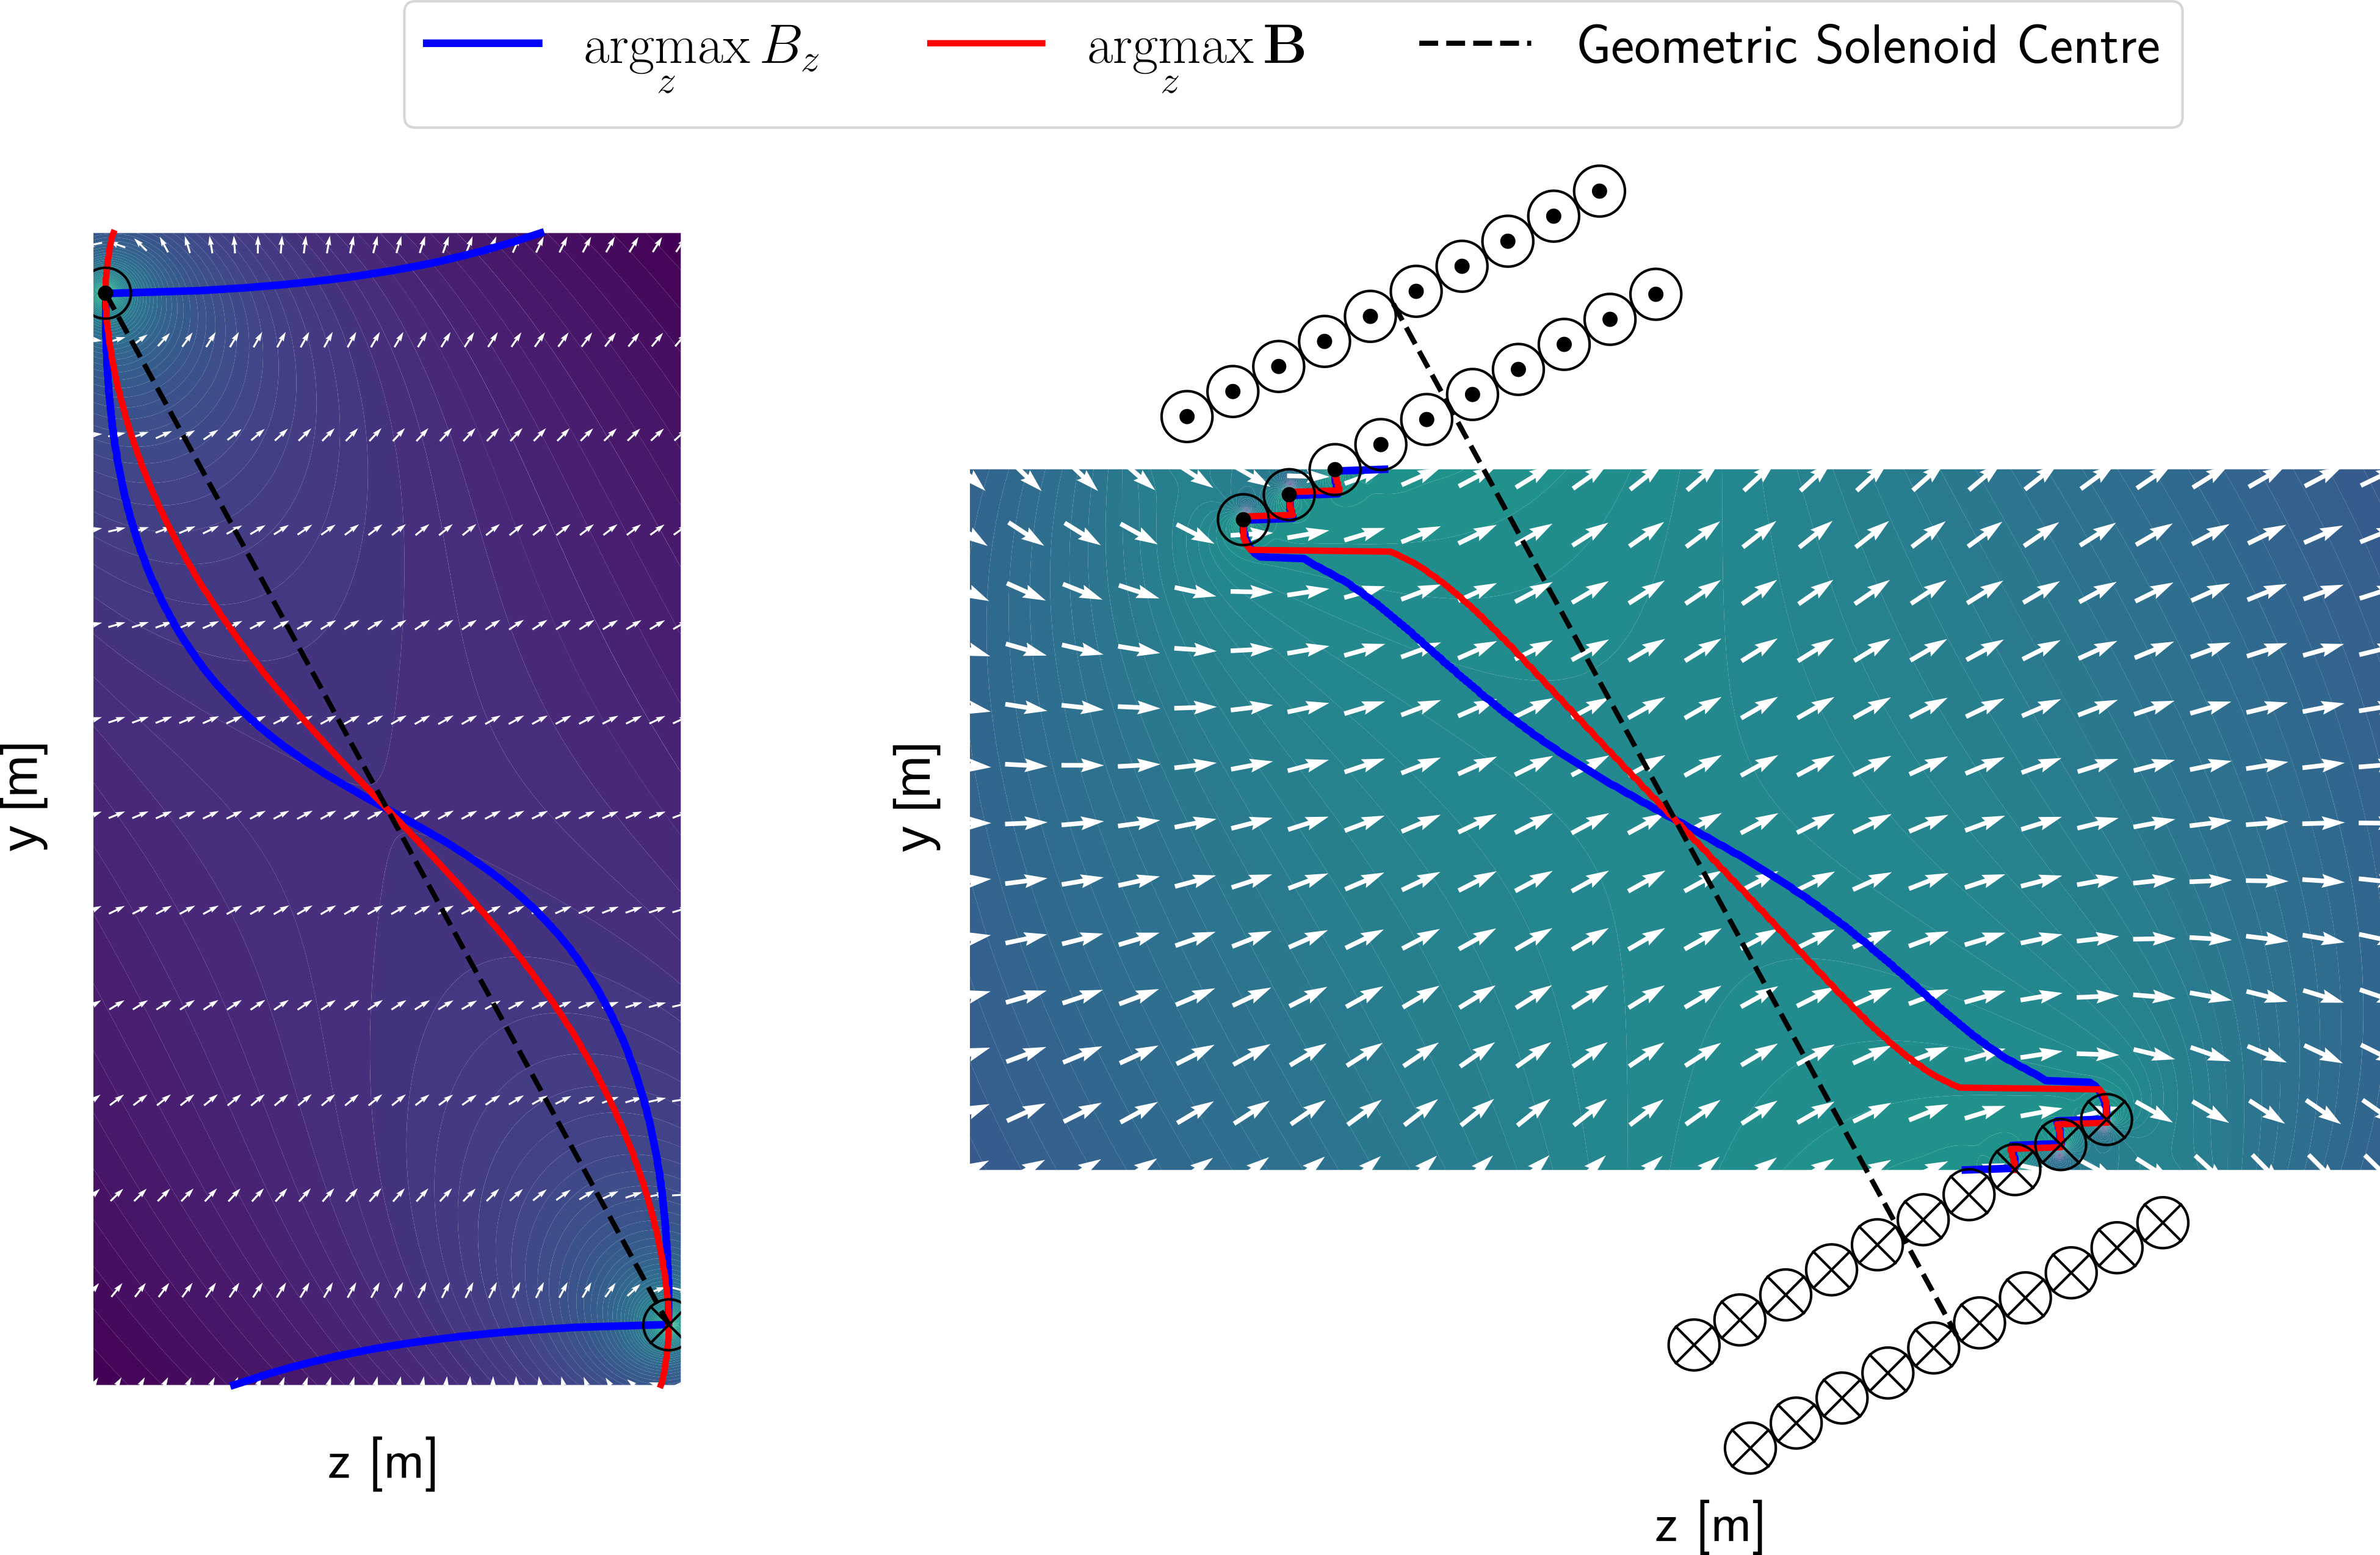
\includegraphics[width=\linewidth]{figs/sim-fieldmap}
    \caption{$\vb{B}$ and $B_z$ argmax over $y$, for a simple current
    loop and coil made up of several current loops. Yaw angle at $500$ mrad.}
    \label{fig:sim-mag-fieldmap-argmax}
\end{figure}

\section{The transversal integral field and dipoles}
\label{sec:dipole-simulations}
In section \ref{sec:theory-dipoles} it was shown that the integral
$B$ field and subsequently the $z$ dipole in field 
series expansions was


\begin{equation}
    \int \limits_{t_0}^{t_1} \vb{B}(\vb{l}(t))dt = C_{0,0}L \approx \mu_0 NI
    \label{eq:Bzlineint}
\end{equation}

for a line integral going through a solenoid, regardless of the yaw
angle $\theta$. $\vb{l}$ is a curve whose image
is a line with length L and whose ends are far from the magnet, where 
the magnetic field strength is negligible.

Now, let $\vb{l}$ be parallel with the $z$ axis, and instead take the
transversal integral fields, as in equations \ref{eq:Bx-Integral} and
\ref{eq:By-Integral}.

\begin{align}
    I_{\vb{l}}(B_x) &:= \int \limits_{\vb{l}} B_x d\vb{l} 
    \label{eq:Bx-Integral}\\
    I_{\vb{l}}(B_y) &:= \int \limits_{\vb{l}} B_y d\vb{l}
    \label{eq:By-Integral}
\end{align}

This could be
likened to measuring the $x$ and $y$ field by translating a hall sensor
through the solenoid, and then taking the integral of the measurements.
It was discovered in the work on this thesis, that the aforementioned
integral fields seems to be connected to the yaw/pitch angle of the 
solenoid.

This relationship can not easily
be found algebraically, and was instead investigated using the same
simulation setup previously described in this chapter. The numerical integral of
both $B_z$ and $B_y$ were taken along $\vb{l}$ over different yaw angles $\theta$.
Like before, the solenoids
radius, length and width were varied, as well as the $x$ and $y$ offset.
The $x, y$ offsets were small enough
for $l$ to pass through the solenoid aperture.

Regardless of all of the variations between simulation passes, the results were
consistent down to a millionth of a radian.
Furthermore, the value of the $By$ integral along $\vb{l}$
was invariant to the $x,y$ location of $\vb{l_1}$ inside the solenoid.
The simulations suggest that when a solenoid is tilted with an angle $\theta$
around the x axis, the integral of $B_y$ along $\vb{l}$ becomes

\begin{equation}
    \int\limits_{\vb{l}}B_y d\vb{l} =
    \tan\left( \frac{\theta}{2} \right)  \int\limits_{\vb{l}}\vb{B} d\vb{l}
    \approx \mu_0\tan\left( \frac{\theta}{2} \right) NI
    \label{eq:tanhalf}
\end{equation}
or alternatively
\begin{equation}
    \frac{I_{\vb{l}}(B_y)}{\mu_0NI} \approx \arctan(\frac{\theta}{2})
    \label{eq:Byint-Error}
\end{equation}

\begin{figure}[h!]
    \centering
    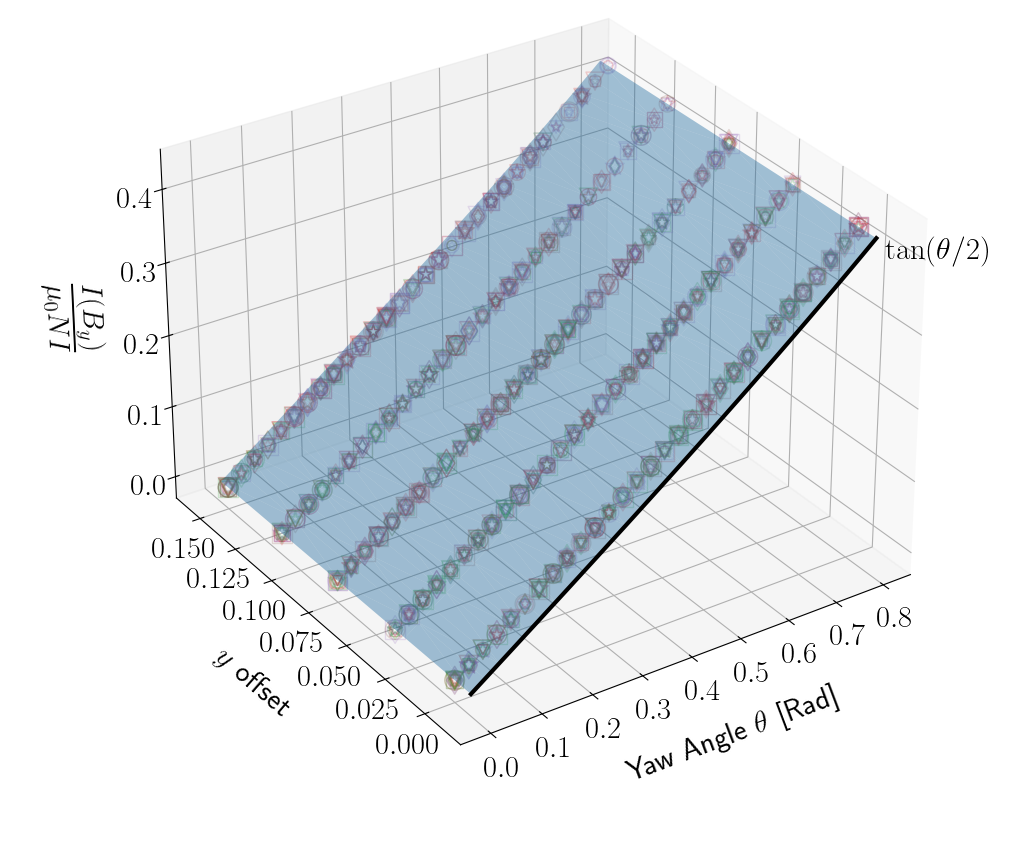
\includegraphics[width=0.8\linewidth]{figs/ByInt3D}
    \caption{Scatter plot with a random subset of simulation results.}
    \label{fig:ByInt3D}
\end{figure}



A randomly chosen subset of the simulation results are plotted in figure \ref{fig:ByInt3D}.
The markers shows the left hand side of equation \ref{eq:Byint-Error} 
as calculated from the simulations and the right hand side is represented by the translucent
blue surface.
Each of the parameters \emph{L}, \emph{W} and \emph{R} are represented
by marker shape, size and color respectively. It can be seen that
equation \ref{eq:tanhalf} holds over all the simulated parameters.

The accuracy is further studied in figure \ref{fig:ByInt-Error},
showing the difference \newline
$\frac{I_{\vb{l}}(B_y)}{\mu_0NI} - \arctan(\frac{\theta}{2})$, which
we will call the error function $E$. Although the error function
is never large in the simulated range of parameters,
it grows with the angle $\theta$.

\begin{figure}[h!]
    \centering
    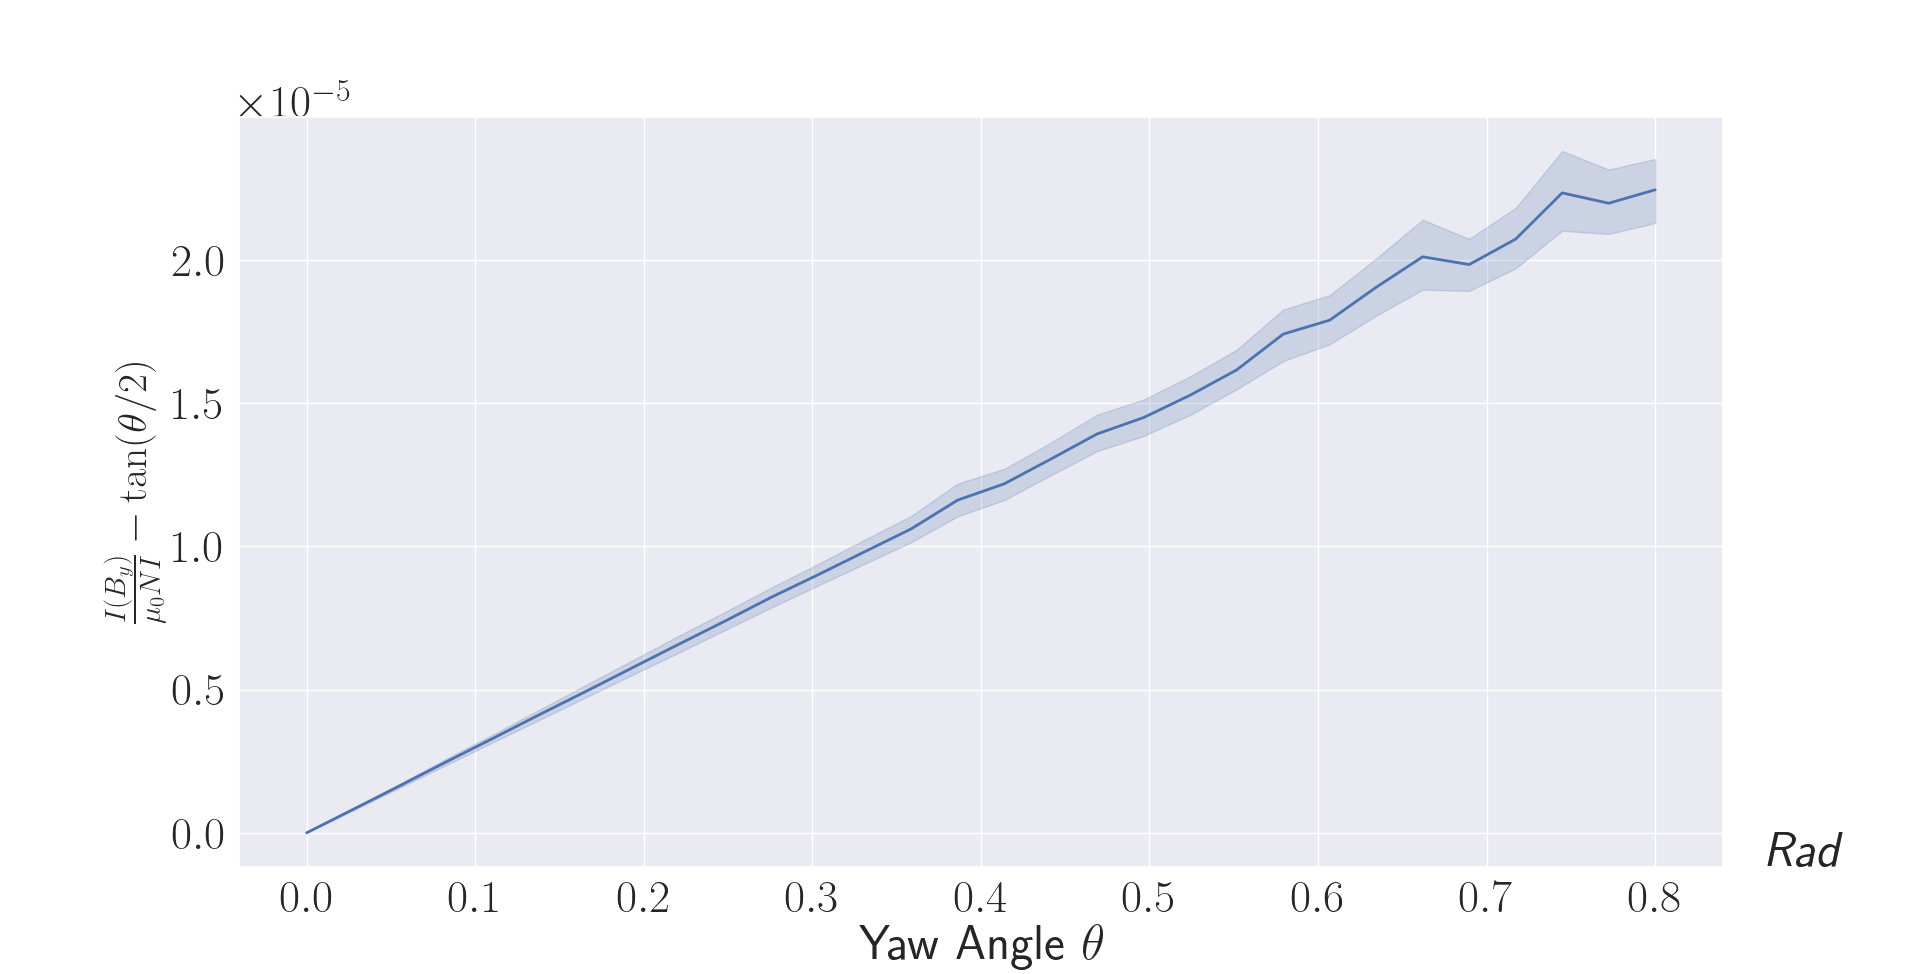
\includegraphics[width=\linewidth]{figs/ByIntError}
    \caption{Plot showing the error function $E$, comparing the simulated results
    with equation \ref{eq:Byint-Error}.}
    \label{fig:ByInt-Error}
\end{figure}


A likely cause is that as the solenoid rotates, the coil windings 
get closer to the line $\vb{l}$ where the integral is evaluated. The 
proximity of the singularities in the windings makes the partial derivative
of the field over $z$ higher, making the discretization errors larger.
To verify this, the error function $E$ was calculated with a single coil
model, this time varying the discretization size instead. As the number
of integration samples grows, the error shrinks up to a point where it  
flattens out, as seen in figure \ref{fig:ByInt-Error-convergence}. It seems
that the limits of the numerical simulations were reached.

\begin{figure}[h!]
    \centering
    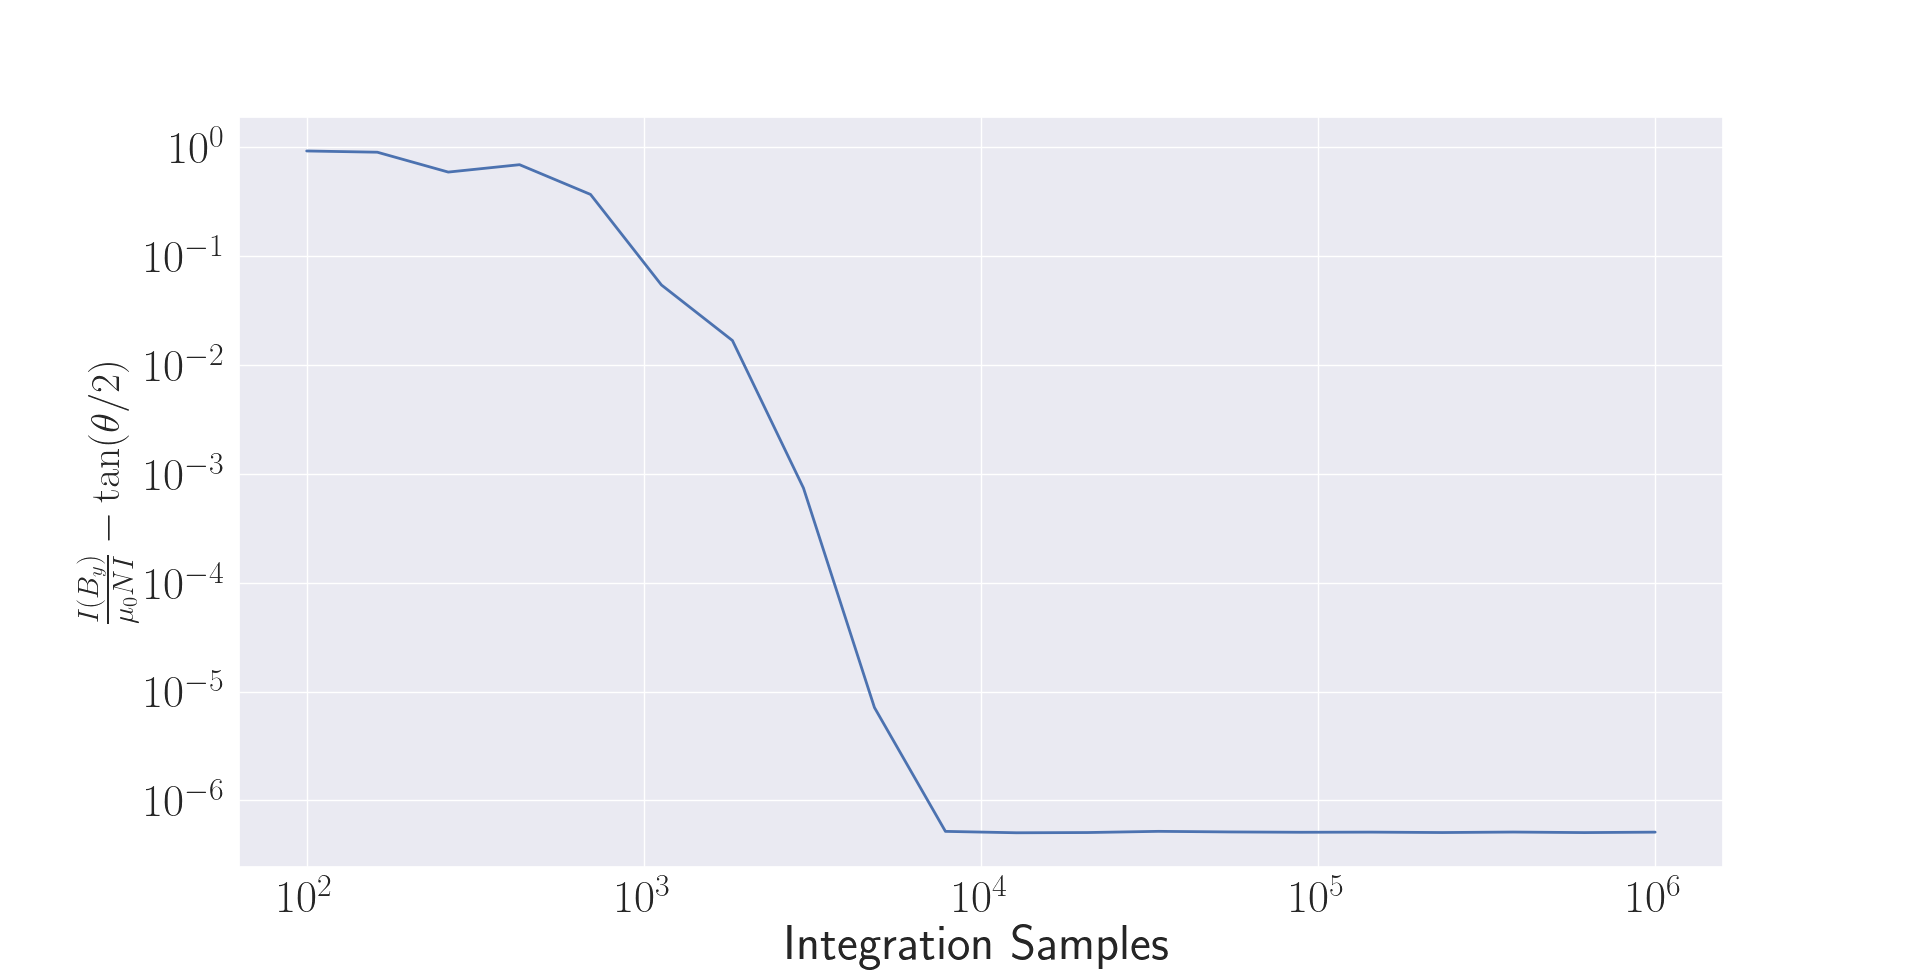
\includegraphics[width=\linewidth]{figs/ByInt-Convergence.png}
    \caption{Plot showing the error function $E$, and how it converges with
    more integration samples.}
    \label{fig:ByInt-Error-convergence}
\end{figure}

Now, looking back at the BFF series from section
\ref{subsubsection:solenoid-harmonics}, specifically the
multipoles in $r$ and $\varphi$, 

\begin{equation}
    \Bffno
\end{equation}

the simulation results presented above can be used to determine
these coefficients. All other components will vanish in the
integrals \ref{eq:By-Integral} and \ref{eq:Bx-Integral} since
$\vb{l}$ spans exactly one period. Furthermore, the
$x$ and $y$ offset do not affect the value of the integral.
This suggests that no higher order multipoles than the dipoles are
created when the solenoid is tilted. Using similar reasoning as 
in equation \ref{eq:Czz}, the following can be said about the 
dipole components in $r, \varphi$ for the BFF series

\begin{align}
    |C_{1,0} + C_{-1,0}| &\approx \mu_0
    \tan\left( \frac{\theta}{2} \right) \frac{NI}{L} \\
    \arg(C_{1,0} + C_{-1,0}) &= \alpha + \frac{\pi}{2}
\end{align}
where $\alpha$ is the angular offset from the $x$ axis to the rotation
axis of the solenoid.
